% \documentclass[man,floatsintext]{apa6}
\documentclass{pnastwo}
\usepackage{pnastwoF}
\usepackage[numbers,sort&compress]{natbib}
% \usepackage[nodoi]{apacite}
\usepackage{graphicx}
\usepackage{amsmath}
\usepackage[american]{babel}
\usepackage[section]{placeins}



%% OPTIONAL MACRO DEFINITIONS
\def\s{\sigma}

%%%%%%%%%%%%
%% For PNAS Only:
\url{www.pnas.org/cgi/doi/10.1073/pnas.xxxxxxxxxx}
\copyrightyear{2008}
\issuedate{Issue Date}
\volume{Volume}
\issuenumber{Issue Number}
%\setcounter{page}{2687} %Set page number here if desired
%%%%%%%%%%%%

% \authornote{Please address correspondence to: 

% \vspace{12 pt}
% Daniel Yurovsky

% Jordan Hall (Building 420)

% Stanford University

% 450 Serra Mall

% Stanford, CA 94305

% \vspace{12 pt}
% Email: yurovsky@stanford.edu 

% \vspace{12 pt}
% Word Count: 1999

% References: 40}

\begin{document}


\title{Synthesizing Accounts of Cross-Situational Learning}
\author{Daniel Yurovsky\affil{1}{Department of Psychology, Stanford University} and Michael C. Frank\affil{2}{Department of Psychology, Stanford University}}
\contributor{Submitted to Proceedings of the National Academy of Sciences
of the United States of America}

% \affiliation{Department of Psychology, Stanford University}
% \shorttitle{Synthesizing Cross-Situational Learning}
% \leftheader{Yurovsky \& Frank}

% \abstract{}

\maketitle


\begin{article}
\begin{abstract}

Co-occurrence statistics between words and objects across situations are a powerful information source for language learners. But, there is considerable debate about how we learn from them. While some theories hold that we accumulate graded, statistical evidence about multiple referents for each word, others suggest that we track only a single candidate referent. In two large-scale experiments with adults, we show that neither account is sufficient: cross-situational learning involves elements of both. Further, the empirical data are captured by a computational model that formalizes how memory and attention interact with both single-referent tracking and statistical accumulation. Together, these data unify opposing positions in a complex debate and underscore the value of understanding the interaction between computational and algorithmic levels of explanation.
\end{abstract}
\keywords{statistical learning, word learning, language acquisition, cognitive development}
\abbreviations{}


\dropcap{N}atural languages are richly structured. From sounds to phonemes to words to referents in the world, statistical regularities characterize the units and their connections at every level. Adults, children, and even infants are sensitive to these statistics, leading to a view of language acquisition as a parallel, possibly implicit, process of statistical extraction \cite{Saffran1996a,Gomez2000}. Recent experiments across a number of domains, however, show that human statistical learning may be significantly more limited than previously believed \cite{Johnson2010c, Yurovsky2012c, Trueswell2013}.

We focus here on the use of statistical regularities to learning the meanings of concrete nouns (known as cross-situational word learning;  \citeNP{Pinker1989, Siskind1996, Yu2007}). Because words' meanings are reflected in the statistics of their use across contexts, learners could discover the meaning of the word ``ball'' (for instance) by noticing that while it is heard across many ambiguous contexts, it often accompanies play with small, round toys. A growing body of experiments shows that adults, children, and infants are sensitive to such co-occurrence information, and can use it to map words to their referents \cite{Yu2007, Smith2008, Scott2012, Vlach2013}.

At \citeauthor{Marr1982}'s \citeyear{Marr1982} computational level, information about a word's meaning can thus be extracted from the environmental statistics of its use \cite{Frank2009a}. However, this computation can be approximated by a number of different algorithmic-level mechanisms, and the one available to humans is under significant debate. Do human learners really maintain a representation of word-object co-occurrences? Some evidence suggests that humans are indeed gradual, parallel accumulators of statistical regularities about the entire system of word-object co-occurrences, simultaneously acquiring information about multiple candidate referents for the same word \cite{Vouloumanos2008, McMurray2012, Yurovsky2014}. Other evidence suggests that statistical learning is a focused, discrete process in which learners maintain a single hypothesis about the referent of any given word. This referent is either verified by future consistent co-occurrences or instead rejected, ``resetting'' the learning process \cite{Medina2011, Trueswell2013}. While both of these algorithmic-level solutions will, in the limit, produce successful word-referent mapping, they will do so very different rates. In particular, if learners track only a singly candidate referent for each word, it may be necessary to posit additional biases and constraints on learners in order for human-scale lexicons to be learned in human-scale time from the input available to children \cite{Vogt2012, Reisenauer2013}.

To distinguish between these two accounts, previous experiments have exposed learners to words and objects in which co-occurrence frequencies indicated several high-probability referents for the same word. At the group level, participants in these experiments showed gradual learning of multiple referents for the same word \cite<e.g.>{Vouloumanos2008, Yurovsky2013}; but gradual, parallel learning curves can be observed at the group level even if individuals are discrete, single-referent learners \cite{Gallistel2004, Medina2011}. Experiments measuring the same learner at multiple points---a stronger test---have produced mixed results. In some cases, learners showed clear evidence of tracking multiple referents for each word, suggesting a distributional approximation mechanism at the algorithmic level \cite{Smith2011a, Yurovsky2013a, Dautriche2014}. In other experiments, however, learners appear to track only a single candidate referent, and to restart from scratch if their best guess is wrong \cite{Medina2011, Trueswell2013}. 

These mixed results expose a fundamental gap in our understanding of the mechanisms by which people encode and track environmental statistics critical for learning language. Because, these experiments differ along a number of dimensions---e.g., methodology, stimuli, timing, and precision of measurement---it is difficult to integrate across them to understand why the algorithmic-level processes underlying statistical learning sometimes appear distributional and sometimes appear discrete \cite<see>[for a review]{Yurovsky2014}.

We hypothesize here that differences in task difficulty may explain differing results across experiments. Two salient dimensions vary across previous studies: ambiguity of individual learning instances, and the interval between successive exposures to the same label. As attentional and memory demands increase, learners may shift from statistical accumulation to single-referent tracking \cite{Smith2011a, Trueswell2013}. We present a strong test of this hypothesis, adapting a paradigm first introduced by \citeA{Bower1963} to study the information learners store in concept identification. We parametrically manipulated both the ambiguity of individual learning trials and the interval between them and measured multiple-referent tracking at the individual-participant level.

Our data show that even at the maximum difficulty tested, adult learners track multiple referents for each word rather than a single referent, providing strong evidence against a qualitative shift from statistical accumulation to single-referent tracking. However, the data also show that learners encode the referents with differing strength, remember much better the one that they hypothesized to be the correct referent. We formalize both the single-referent and statistical accumulation models, as well as an integrative model that subsumes both as special cases along a continuum. Only the integrative model can account for the data. We then show that this model makes nearly perfect parameter-free predictions for a follow-up experiment designed to determine the extent to which learners encode mappings rather than individual words and objects. We conclude that cross-situational word learning is best characterized by an integrative account: Learners track both a single target referent and an approximation to the co-occurrence statistics, but the strength of this approximation varies with the complexity of the learning environment (Figure~\ref{fig:design}b). 

 \begin{figure}[t]
	\center{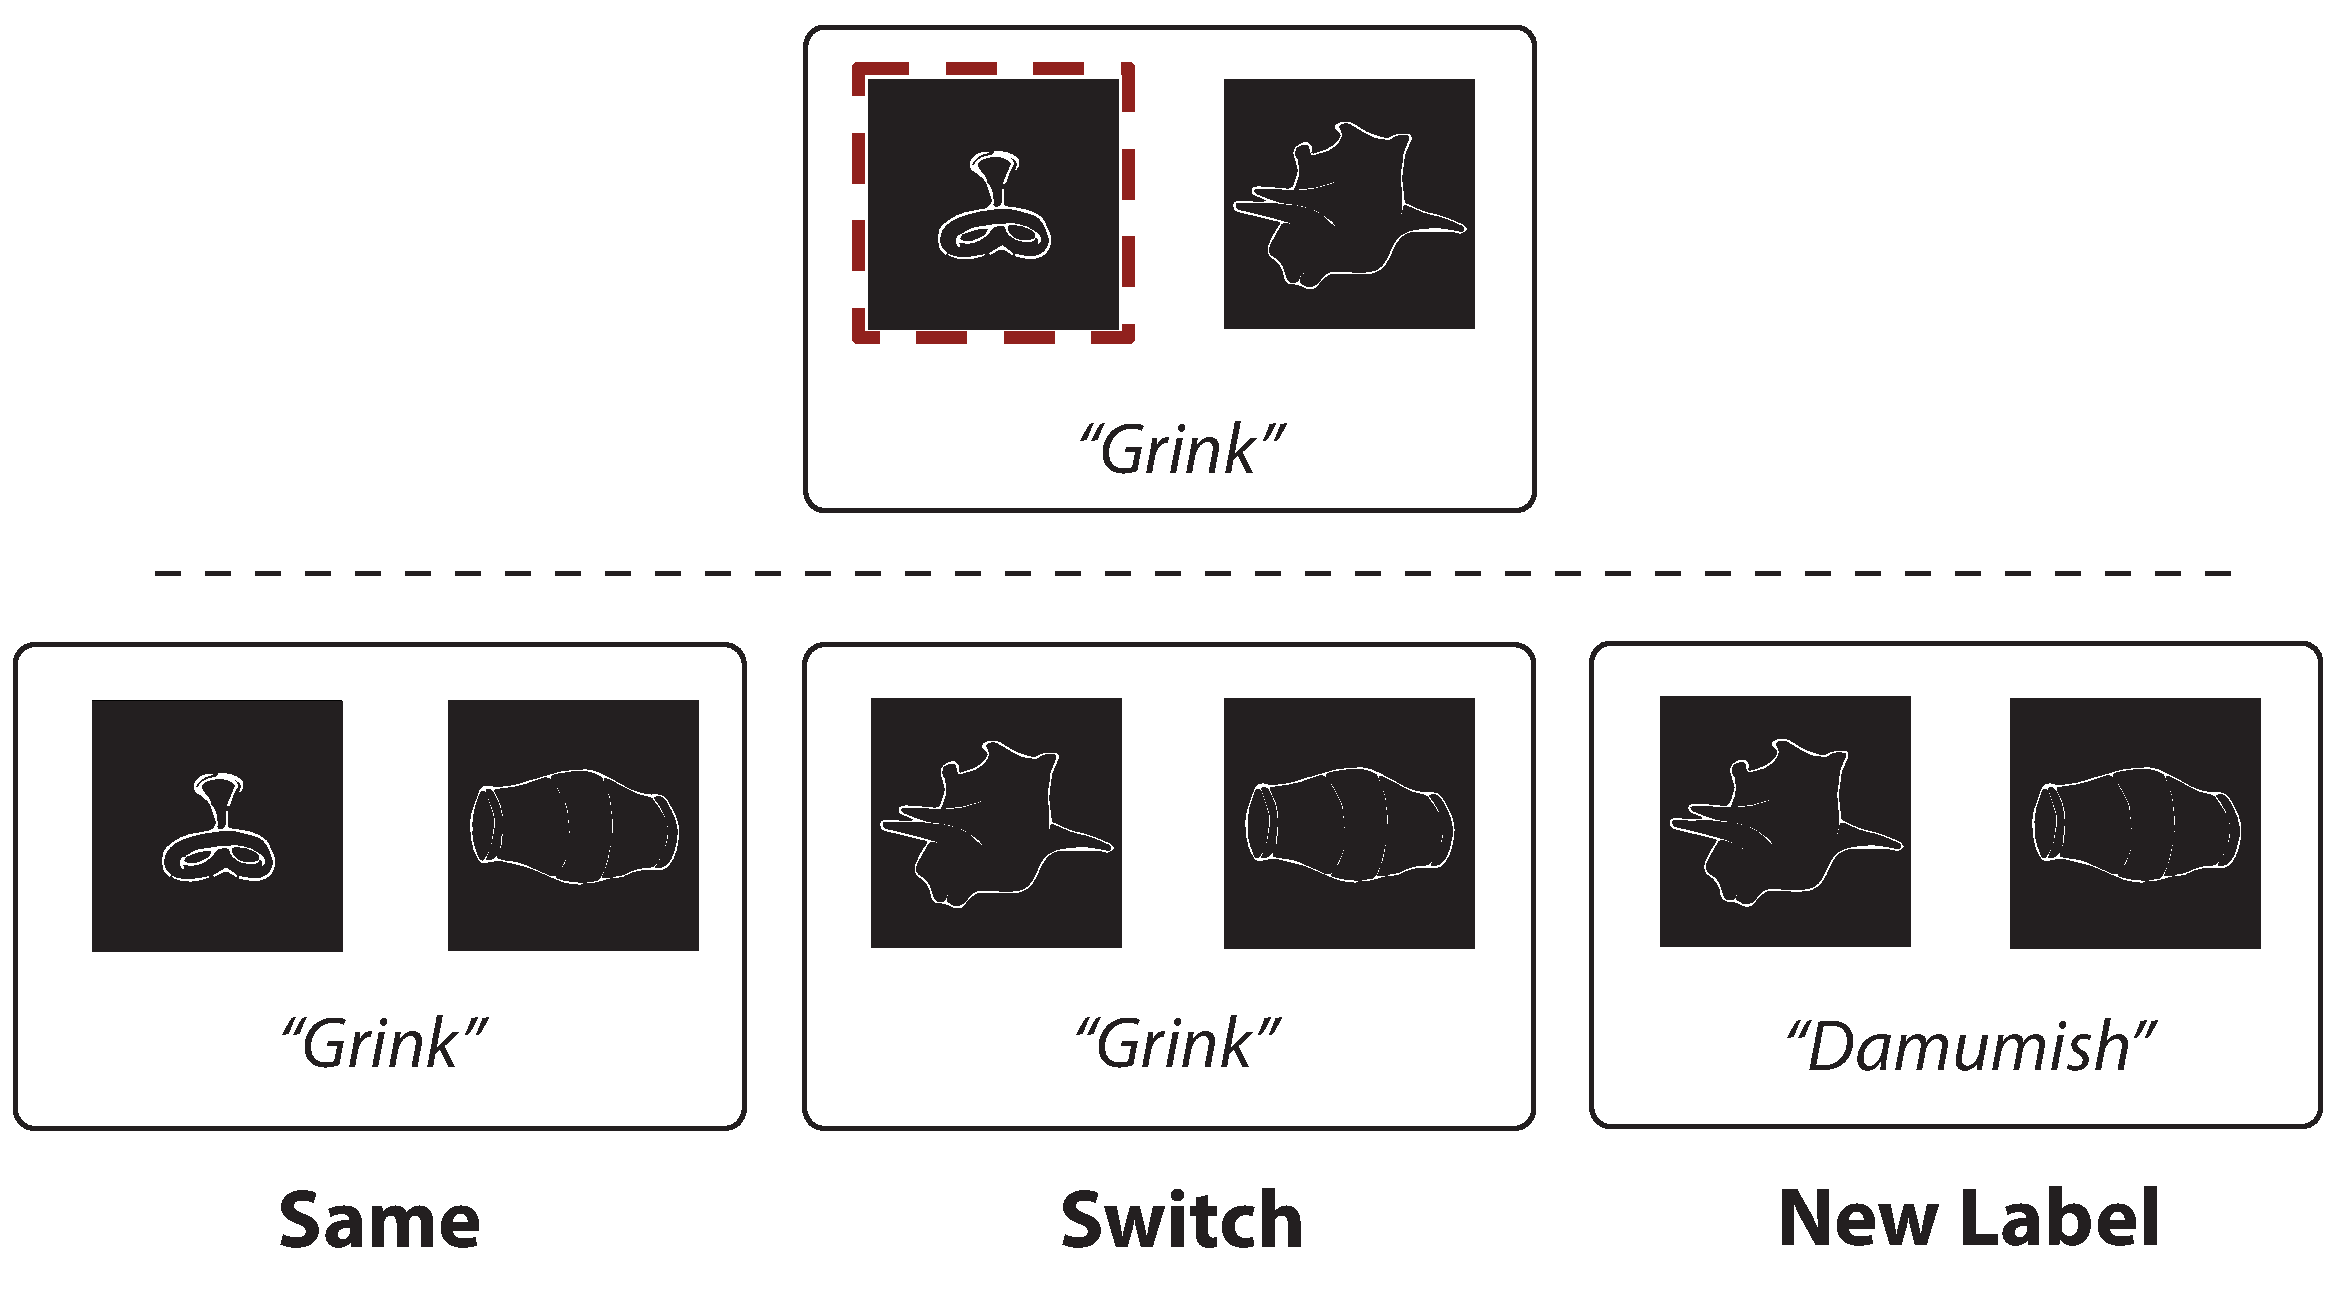
\includegraphics[width=3.4in]{figures/design_fig}}
	\caption{\label{fig:design} (a)  A schematic of the experimental trials seen by participants in Experiments 1 and 2. On their first exposure to each novel word, participants were asked to guess its correct referent. In Experiment 1, the second trial for each word was either a Same trial---the set of referents contained the participant's previous hypothesis, or a Switch trial---the set of referents contained one the participant had previously \emph{not} hypothesized. In Experiment 2, Switch trials were replaced with New Label trials that showed same set of referents but a played a novel word. The number of referents on the screen and the interval between successive exposures to the same word varied across conditions. (b) A representation of the continuum between the statistical accumulation and single-referent tracking models as learners' attention is varied from evenly distributed ($\sigma=\frac{1}{|O|}$) to focused on a single referent ($\sigma=1$), as well as the best-fitting integrated model's position along this continuum.}
\end{figure}

\section{Experiment 1}

We designed Experiment 1 to estimate learners' memory for both their single best hypothesis about the correct referent of a novel word and their additional statistical knowledge as demands on attention and memory varied. Participants saw a series of individually ambiguous word learning trials in which they heard one novel word, viewed multiple novel objects, and made guesses about which object went with each word. To succeed, participants needed to encode at least one of the objects that co-occurred with a word, remember it until their next encounter with that word, and check whether that same object was again present. If participants encoded exactly one object, they would succeed only when their initial hypothesis was correct. However, the more \emph{additional} objects participants encoded on their first encounter with a word, the greater their likelihood of succeeding even if their initial hypothesis was incorrect. 

Rather than allowing chance to determine whether participants held the correct hypothesis on their first exposure to a novel word, the set of novel objects presented on the second exposure to each word was constructed based on participants' choices. On \emph{Same} trials, the participant's hypothesized referent was pitted against a set of novel competitors. In contrast, on \emph{Switch} trials, one of the objects the participant had previously \emph{not} hypothesized was pitted against a set of novel competitors (see Figure~\ref{fig:design}a). Logically, either a single-referent tracking or a statistical accumulation mechanism will succeed on Same trials. However, only statistical accumulation of information about non-target items can allow participants to succeed on Switch trials.

\subsection{Method}

\subsubsection{Participants}

Experiment 1 was posted to Amazon Mechanical Turk as a set of Human Intelligence Tasks (HITs) to be completed only by participants with US IP addresses that paid 30 cents each \cite<for a detailed comparison of laboratory and Mechanical Turk studies see>{Crump2013}. Ninety HITs were posted for each of the 16 Referent x Interval conditions for a total of 1440 paid HITs. If a participant completed the experiment more than once, he or she was paid each time but only data from the first HIT completion was included in the final data set (excluded 180 HITs). In addition, data was excluded from the final sample if participants did not give correct answers for familiar trials (64 HITs, see Design and Procedure). The final sample thus comprised 1,196 unique participants, approximately 75 participants per condition (range: 71-81).

\subsubsection{Stimuli}

Stimuli for the experiment consisted of black and white pictures of familiar and novel objects and audio recordings of familiar and novel words. Pictures of 32 familiar objects spanning a range of categories (e.g. squirrel, truck, tomato, sweater) were drawn from the set constructed by \citeA{Snodgrass1980}. Pictures of distinct but difficult to name novel objects were drawn from the set of 140 first used in \citeA{Kanwisher1997}. For ease of viewing on participants' monitors, pixel values for all pictures were inverted so that they appeared as white outlines on black backgrounds (see Figure~\ref{fig:design}a). Familiar words consisted of the labels for the familiar objects as produced by AT\&T Natural Voices$\texttrademark$ (voice: Crystal). Novel words were 1-3 syllable pseudowords obeying the rules of English phonotactics produced using the same speech synthesizer. 
\subsection{Design and Procedure}

Participants were exposed to a series of trials in which they heard a word, saw a number of objects, and were asked to indicate their guess as to which object was the referent of the word. After a written explanation of this procedure, participants were given four practice trials to introduce them to the task. On each of these trials, they heard a Familiar word and saw a line drawing of that object among a set of other familiar objects. On the first two trials, participants were asked to find the squirrel, and the correct answer was in the same position on each trial. On the next two trials, participants were asked to find the sweater, and the correct answer switched positions from the first to the second trial (in order to ensure that participants understood the on-screen position was not an informative cue to the correct target). These trials also served to screen for participants who did not have their audio enabled or who were not attending to the task.

After these Familiar trials, participants were informed that they would now hear novel words, and see novel objects, and that they should continue selecting the correct referent for each word. Participants heard each of the eight novel words twice, but the order in which these words were presented and the number of objects seen on the screen were varied across sixteen between-subjects conditions. Participants saw either 2, 3, 4, or 8 Referents on each trial, and the two trials for each word occurred either back-to-back, or were interleaved between trials for other words for an Interval of 1, 2, 3, or 8. Four of these follow-up trials were Same trials in which the referent that participants selected on the first encounter with that object appeared again amongst the set of objects. The other four were Switch trials in which one of the referents in the set was selected randomly from the objects a participant \emph{did not} select on the previous exposure to that word. All other referents were completely novel on each trial. The number of referents on Familiar trials for each participant matched the number of referents they would see on Same and Switch trials.

Because participants performed this task over the internet, it was important to indicate to them that their click had been registered. Thus, a red dashed box appeared around the object they selected on for 1 second after their click was received. This box appeared around the selected object whether or not it was the ``correct'' referent.\footnote{It is possible that forcing participants to select an object on each trial could have changed their performance. However, control conditions from three previous experiments suggest that empirically this is not the case \cite{Medina2011, Smith2011a, Trueswell2013}.}

\subsection{Results}

Do statistical learners encode multiple referents for each word, or do they instead encode only a single hypothesized referent? We compared the distribution of correct responses made by each participant to the distribution expected if participants were selecting randomly (defined by a Binomial distribution with four trials and a probability of success of  $\frac{1}{\#Referents}$). The top row of Figure~\ref{fig:exp1_2_data} shows participants' accuracies in identifying the referent of each word in all conditions for both kinds of trials (Same and Switch). At all Referent and Interval levels, both for Same and for Switch trials, participants' responses differed from those expected by chance (smallest $\chi^{2}(4) = 15.07$, all $p < .01$). Thus, adults encode more than a single hypothesis in ambiguous word learning situations, even under high levels of memory and attentional load. 

Next, to quantify the effect of each factor on word learning, we fit a mixed-effect logistic regression model to the data from the full dataset \cite{Baayen2008}. This analysis showed significant main effects of Number of Referents, Interval, and Trial Type. In addition, the model showed a significant two-way interaction between Referents and Trial Type and a significant three-way interaction between all three factors (see Supporting Material). Thus, while word learning was best at low levels of referential ambiguity and at low memory demands, the decreases in word learning observed on Same and Switch trials were due to different factors. For Same trials, the number of Referents played a relatively small role in the difficulty of learning, while the Interval between learning and test played a large role. However, for Switch trials, there was relatively little decline in word mapping as Interval increased but a large decline due to number of Referents. 

\begin{table}
\begin{center}
\begin{tabular}{lrrrrl}
\hline
Predictor & Estimate & Std. Error & $z$ value & $p$ value & \\
\hline
Intercept & 4.69 & 0.43  & 10.98 &  <0.0001 & ***  \\
Log(Referents)  & -.55 & .20  & -2.80 &  <0.01 & **   \\
Log(Interval)  & -.42 & .20  & -2.08 &  <0.05 & *  \\
Switch Trial  & -1.46 & .44  & -3.30 &  <0.0001 & ***   \\
Log(Referents)*Log(Interval)  & -.13 & .09 & -1.38 &  .17 &  \\
Log(Referents)*Switch  & -1.03 & .21 & -5.00 &  <0.0001 & ***   \\
Log(Interval)*Switch  & .14 & .21  & .67 &  .50 &  \\
Log(Refs) * Log(Int)*Switch  & .20 & .10  & 2.02 &  <0.05 & *  \\
\hline
\end{tabular}
\end{center}
\caption{\label{tab:exp1_reg}Predictor estimates with standard errors and significance information for a logistic mixed-effects model predicting word learning in Experiment 1. The model was specified as \small{\tt{Correct \textasciitilde \hspace{1pt} Log(Referents) * Log(Interval) * TrialType + (TrialType | subject)}}.}
\end{table}

 \begin{figure*}[t]
	\center{\includegraphics[width=\textwidth]{figures/exp1_data}}
	\caption{\label{fig:exp1_2_data} Proportion of repeated referents selected by participants at each combination of number of Referents and Interval on Same and Switch trials in Experiment 1. Each datapoint represents ~75 participants  and error bars indicate 95\% confidence intervals computed by non-parametric bootstrap. Curves indicate the fit of a linear mixed model. Learning in all conditions of Experiment 1 differed from chance and declined mostly due to Interval for Same trials but mostly due to Referents for Switch trials.} 
\end{figure*}

\begin{table}
\begin{center}
\begin{tabular}{lrrrr}
\hline
Model & Log Likelihood &BIC & E1 $r^{2}$ & E1+2 $r^{2}$ \\
\hline
Statistical Accumulation & -5924 & 11863 & .32  & .67\\
Single Referent & -5337 & 10690 & .83 & .77 \\
\textbf{Integrated} & \textbf{-4854} & \textbf{9733} & \textbf{.95}  & \textbf{.98}\\
\hline
\end{tabular}
\end{center}
\caption{\label{tab:model}Likelihood and Correlation measures for models on Experiments 1 and 2. The Integrated model outperformed both of the individual accounts on all measures.}
\end{table}

%integrated
%> model.sigma
%[1] 0.5653685
%> model.lambda
%[1] 0.1597503
%> model.gamma
%[1] 1.609619

%guess
%> model.lambda
%[1] 0.1611523
%> model.gamma
%[1] 0.9107275

%parallel
%> model.lambda
%[1] 0.1029245
%> model.gamma
%[1] 1.776237

\section{Experiment 2}

Participants' above-chance accuracy on Switch trials in Experiment 1 provides evidence of their memory for multiple objects, but not necessarily for the formation of referential mappings between the objects and the novel words. That is, participants could have succeeded despite ignoring the words by simply selecting the most familiar object on each trial. To rule out this explanation, Experiment 2 replaced Switch Trials with New Label trials in which participants saw an object they had previously \emph{not} selected among a set of novel competitors but heard a \emph{New Label}.
If the underlying mechanism for tracking multiple referents is pure referent familiarity, New Label trials should produce similar responses to the Switch trials in Experiment 1. In contrast, if success on Switch trials was due to a mapping between words and referents, New Label trials should show a different pattern of performance.

\subsection{Method}

\subsubsection{Participants}

As in Experiment 1, participants for Experiment 2 were recruited from Amazon Mechanical Turk under the constraint that they had a US IP address. Each HIT paid 30 cents for completion. Sixty HITs were posted for each of the sixteen Referent x Interval conditions for a total of 960 paid HITs. Participants were again paid for multiple HITs, but only data from their first was included in the final set (excluded 100 HITs). In addition, data was again excluded from the final sample if participants did not give correct answers for familiar trials (60 HITs). The final sample thus comprised 803 unique participants, approximately 50 participants per condition (range: 41--55).

\subsection{Stimuli, Design, and Procedure}

All aspects of the Stimuli, Design, and Procedure of Experiment 2 were identical to those of Experiment 1 except for the construction of New Label trials. On these trials, the set of candidate referents was the same as on Switch trials in Experiment 1, but the word was novel (Figure~\ref{fig:design}a).

\subsection{Results}

Participants showed robust evidence of learning mappings (rather than simply tracking familiar objects). Whereas participants on Same trials were more likely than predicted by chance to select a referent they had previously seen but not guessed, participants in New Label trials were, in many cases, \emph{less} likely than predicted by chance to select these same referents. Further, in all Referent and Interval conditions, performance on New Label trials differed significantly from performance on comparable Switch trials. That is, these participants recognized these referents from their first exposure, and further recognized that they did not co-occur on their previous exposure with the label they heard at test (bottom row of Figure~\ref{fig:exp1_2_data}).

In addition, a mixed-effects logistic regression largely reproduced the patterns observed in Experiment 1 -- word learning accuracies on Same trials declined predominantly due to Interval between learning and test, and very little due to the number of Referents. New Label trials were driven almost entirely by the number of Referents---as was the case with Switch trials in Experiment 1.

\begin{table}
\begin{center}
\begin{tabular}{lrrrrl}
\hline
Predictor & Estimate & Std. Error & $z$ value & $p$ value & \\
\hline
Intercept & 3.97 & 0.25  & 16.01 &  <0.0001 & ***  \\
Log(Referents)  & -.48 & .09  & -4.85 &  <0.001 & ***   \\
Log(Interval)  & -.60 & .07  & -8.57 &  <0.001 & ***  \\
New Label Trial  & -4.03 & .28  & -14.09 &  <0.0001 & ***   \\
Log(Referents)*Switch  & -.24 & .12  & -1.98 &  <.05 & * \\
Log(Interval)*New Label  & .58 & .08 & 7.13 &  <0.0001 & ***   \\
\hline
\end{tabular}
\end{center}
\caption{\label{tab:exp2_reg}Predictor estimates with standard errors and significance information for a logistic mixed-effects model predicting word learning in Experiment 2. The model was specified as \small{\tt{Correct \textasciitilde \hspace{1pt} Log(Referents) * TrialType + Log(Interval) * TrialType + (TrialType | subject)} }}
\end{table}


%  \begin{figure*}[!t]
% 	\center{\includegraphics[width=\textwidth]{figures/exp2_data}}
% 	\caption{\label{fig:exp1_2_data} Proportion of repeated referents selected by participants at each combination of number of Referents and Interval on Same and Switch trials in Experiment 1. Each datapoint represents ~50 participants  and error bars indicate 95\% confidence intervals computed by non-parametric bootstrap. Curves indicate the fit of a linear mixed model.} 
% \end{figure*}

Finally, we can use the models presented above, with parameters estimated from Experiment 1, to make parameter-free predictions about the New Label condition. As before, the Single Hypothesis and Parallel Accumulation models predict some of the variance in the new data, but leave much unexplained. With parameter values fixed to those estimated for Experiment 1, the Integrated model makes near-perfect predictions about the new data however, explaining 98\% of the combined variance in the data from Experiments 1 and 2 (Table~\ref{tab:model}). Figure~\ref{fig:model_fit} presents model predictions for all of the data collected. Taken together, Experiments 1 and 2 thus provide strong evidence that adults track not only a single hypothesis for the most likely referent of a novel word, but also some approximation to distributional statistics.

Our data suggest that neither the single-referent tracking nor the statistical accumulation account of cross-situational word learning can be correct. Instead, it appears that cross-situational word learning is best characterized by a combination of both of these mechanisms. In the next section, we formalize this idea.

\section{Model}

We begin by describing the computational-level learning problem posed by Experiment 1 using the model developed by \citeA{Frank2009a}. In this framework, the learner observes a set of situations $S$ with the goal of determining the lexicon of word-object mappings $L$ that produced them $P(L|S)$. Each of these situations consists of two observed variables: objects ($O$) and words ($W$). In addition, situations implicitly contain an additional hidden variable: an intention ($I$) by the speaker to refer to one of the objects. Thus, from the set of objects present in the situation, the speaker first chooses one to refer to and then produces its word label. 

We can use Bayes' rule to determine the inferential computation the learner must perform: 

\begin{align} 
P(L|S) \propto & \;P(S|L) \: P(L) \label{eq:wurwur1}
\end{align}

\noindent Each trial in our experiment consisted of a word and a set of objects. We model the unobserved link between the word and one of the objects as $I$, the referential intention. Thus, the probability of the lexicon is given as:

\begin{align}
P(L|S) \propto & \prod\limits_{s\in{S}}P(W_{s},I_{s}, O_{s},|L) \: P(L) \label{eq:wurwur2}
\end{align}

\noindent Because the referential intention mediates the relationship between words and objects \cite{Frank2009a}, we can rewrite this using the chain rule as:

\begin{align}
P(L|S) \propto & \prod\limits_{s\in{S}}P(W_{s}| I_{s}, L) \: P(I_{s}|O_{s})  \: P(L) \label{eq:wurwur3}
\end{align}

To make predictions from this model, we need to define the probabilities in Equation~\ref{eq:wurwur3}. Following \citeA{Frank2009a}, we propose that the word  ($W$) used to label the intended referent on each trial is chosen uniformly from the set of all words in the lexicon for that object ($L_{o}$). In addition, we propose a simple parsimony prior for the lexicon. A priori, the larger the set of words in the lexicon that refer to the same object $O$, the lower the probability of that lexicon: $P(L_{o}) \propto \frac{1}{|L_{o}|}$. 

We can then take this computational-level description of the problem and add cognitive constraints to provide an algorithmic-level account of learning \cite<see e.g.>{Frank2010a, Shi2010}. We start by defining the learner's beliefs about $P(I|O)$, the probability of the speaker choosing to refer to each object in the set. One possibility is to let each object be equally likely to be the intended referent, implementing parallel Statistical Accumulation as in \citeA{Frank2009a}. Alternatively, the learner could place all of the probability mass on one hypothesized referent -- implementing a Single Referent tracking strategy. A more flexible alternative is to assign some probability mass $\sigma$ to the hypothesized referent, and divide the remainder evenly among the remaining objects: $\frac{1-\sigma}{|O|-1}$. This Integrated model subsumes the other two as special cases: At $\sigma=1$, it becomes a Single Referent tracker, and at $\sigma=\frac{1}{|O|}$, it becomes a parallel Statistical Accumulator (Figure~\ref{fig:design}b).

Next, we model how learners' memories for observed situations decay over time. We follow previous memory researchers by formalizing memory for a lexical entry as a \emph{power function} of the interval between successive exposures, where $\gamma$ scales the strength of initial encoding and $\lambda$ defines the rate of decay \cite{Anderson1991a}.

\begin{align}
M(L_{o}) = \gamma \, L_{o} \, t^{-\lambda}
\end{align}

Finally, we provide a choice rule for describing how learners select at test among the objects on each trial. We propose that learners choose the correct referent with probability proportional to their memory for its lexical entry, and otherwise choose randomly among the set of referents.\footnote{This formulation is equivalent to using \citeauthor{Luce1959}'s \citeyear{Luce1959} Choice Axiom in which the target has strength  $M(L_{o}) + \frac{1-M(L_{o})}{|O|}$ and each foil has strength $\frac{1-M(L_{o})}{|O|}$.}

\begin{align}
P(Correct) = M(L_{o}) + \frac{1-M(L_{o})}{|O|}
\end{align}

All 3 models---Statistical Accumulation, Single Referent, and Integrated---were fit to the data from Experiment 1 at the individual-participant level. While the Single Referent and Statistical Accumulation models capture some of the structure in the data, each leaves significant variance unexplained. The Single Referent Model cannot predict above-chance performance on Switch trials, and the Statistical Accumulation model cannot predict a difference between the Same and Switch trials. The Integrated model, however, predicts 95\% of the variance in the data, and significantly outperforms the other models in BIC comparisons as well---a metric that trades off its superior performance against its one additional parameter. Table~\ref{tab:model} shows statistics of fit for all models.

 \begin{figure}[!tb]
	\center{\includegraphics[width=\textwidth]{figures/exp1and2fit}}
	\caption{\label{fig:model_fit} Predictions of the Integrated model for all conditions in Experiment 1 and 2. The model was able to account for 98\% of the variance in the data, significantly outperforming both the Single Hypothesis and Parallel Accumulation models.}
\end{figure}

\section{General Discussion}

For an ideal learner, word-object co-occurrence statistics contain a wealth of information about meaning. But how is this information used by human learners? One possibility is that learning is fundamentally statistical, and we gradually accumulate distributional information across situations. Another possibility, however, is that we track only a single, discrete hypothesis at any time. While each of these accounts has some support in prior work, neither is consistent with all of the extant data.

Our results here suggest an explanation: The degree to which learners represent statistical information depends on the complexity of the learning situation. When there are many possibilities, learners represent little about any other than the one that is currently favored; when there are few, learners represent more. This account does not depend on positing multiple, discrete learning systems. Instead, the tradeoff between the most likely hypothesis and the alternatives emerges from graded constraints on memory and attention. Consistent with this account, when we manipulated the cognitive demands of a cross-situational word learning paradigm, we found a gradual shift in the fidelity with which alternatives were represented (Experiments 1 and 2).

The graded shift in representation we found was well-described by an ideal learning model, but only when this model was modified to take into account psychological constraints. The algorithmic instantiation of these constraints that best fit the data was intermediate between the two extreme poles of parallel statistical accumulation and single-referent tracking. This unifying account provides a route by which both hypotheses and sensitivity to statistics can make complementary contributions to word learning \cite{Waxman2009,Kachergis2013}. 

The shift from a computational to an algorithmic level of description was critical in capturing the pattern of human performance in our task \cite{Marr1982,Frank2010a,Yurovsky2012c}. For the current model, we chose one principled instantiation of cognitive limitations based on previous work, but there may be other consistent proposals. Our model was not overfit to the particular data we collected, however: Based on data from Experiment 1, we used our model to make parameter-independent predictions about human performance that were supported in Experiment 2.

Where do children sit along this continuum from statistical learner to discrete hypothesis tester? In our paradigm---which presents learners with only a single piece of evidence---the youngest children we tested showed no sign of tracking multiple referents. In contrast, older preschoolers showed increasingly more success. While this developmental shift could signal a genuine discontinuity, our modeling work suggests that it also might emerge gradually via developmental changes in attention and memory \cite{Yu2011a,Vlach2013}.

It remains a question for future work how these developmental findings relate to young children's word learning outside of the lab. In natural speech to children, referents are introduced into common ground and then discussed \cite{Clark2003}. In contrast, tasks such as ours are intentionally stripped of the constellation of communicative, attentional, and linguistic cues that typically surround naming events \cite{Frank2013a, Gogate2010, Mintz2003}, and objects are presented only a single time, rather than embedded in a coherent discourse \cite{Frank2013a, Rohde2013}. These differences suggest that children could track multiple alternative referents at a different level in their natural environment than they did in our task. Nonetheless, our results provide both an empirical and theoretical starting point for measuring children's word learning in more naturalistic contexts.

Our work shows how ideal learning models can inform psychological accounts of statistical learning more broadly. Although we focused here on noun learning, our results are relevant to work on many aspects of early language, including phonetic category learning, speech segmentation, and grammar learning. In each of these domains, researchers have debated the degree to which learners represent distributional information \cite{Endress2005, Frank2010a, McMurray2013}. We suggest a synthesis. Learning is fundamentally distributional, but the fidelity of learners' distributional estimates depends critically on their limited attention and memory.

\section{Author Contributions}

DY and MCF designed the research, DY performed the experiments and analyzed the data, DY and MCF wrote the paper.

\section{Acknowledgements}

%We are grateful to Sarah Case and Janelle Klaas for help with data collection and to Linda Smith, Elika Bergelson, Molly Lewis, Ann Nordemeyer, and all of the members of the Language and Cognition Lab for their feedback on this project. In addition, we thank the parents, children, and staff at the San Jose Children's Discovery Museum for supporting us in collecting developmental data. 

This work was supported by a NIH NRSA F32HD075577 to DY as well as grants from the Merck Scholars Foundation and the Stanford Center Health Research Initiative to MCF.

\bibliographystyle{unsrtnat}
\bibliography{library11}

\end{document}
